\chapter{Fluorescent neuronal cells dataset}
\label{chap:partI_dataset}

% \savegeometry{origigeom}
% \clearpage
% \newgeometry{lmargin=2cm}
\begin{figure}%[!b]
\begin{subfigure}{0.5\textwidth}
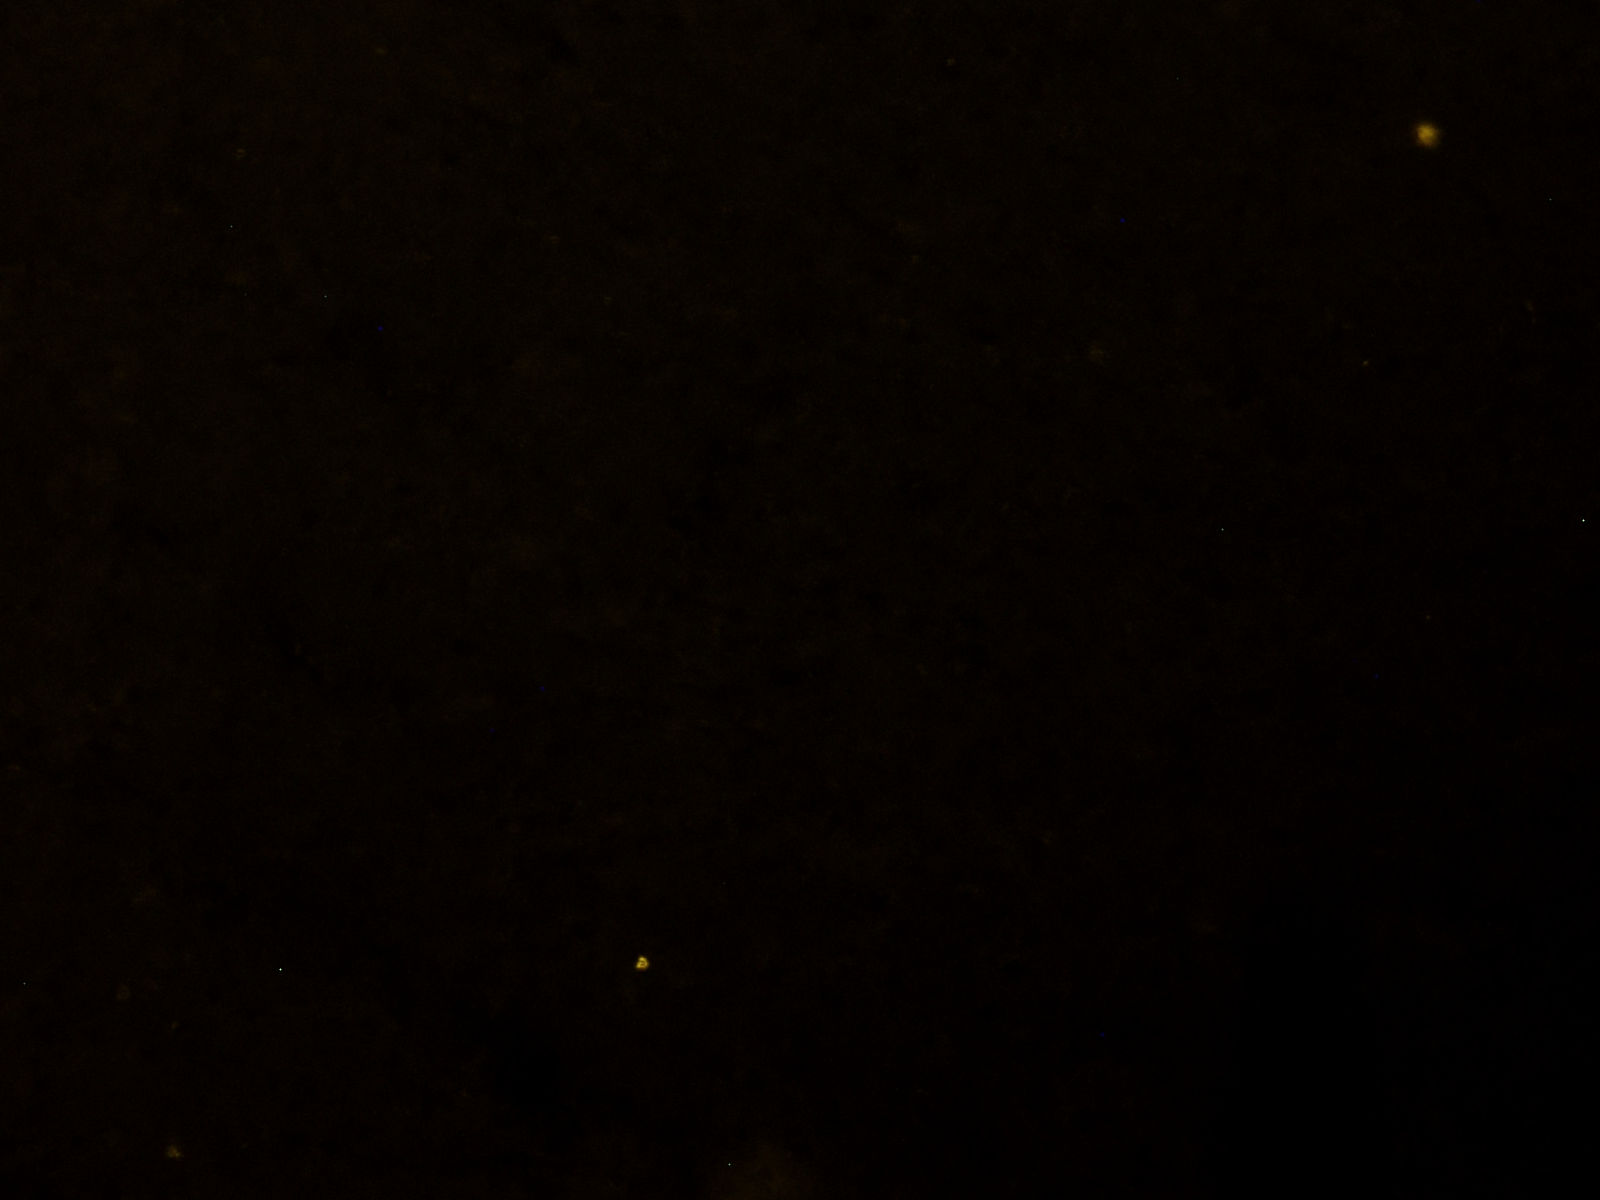
\includegraphics[width=\linewidth]{figures/120_dataset/i_empty.png}
\subcaption{empty}\label{fig:dataset:empty}
\end{subfigure}
\begin{subfigure}{0.5\textwidth}

\includegraphics[width=\linewidth]{figures/120_dataset/m_empty.png}
\subcaption{mask}\label{fig:dataset:empty_mask}
% \label{fig:dataset:empty}
\end{subfigure}

\begin{subfigure}{0.5\textwidth}
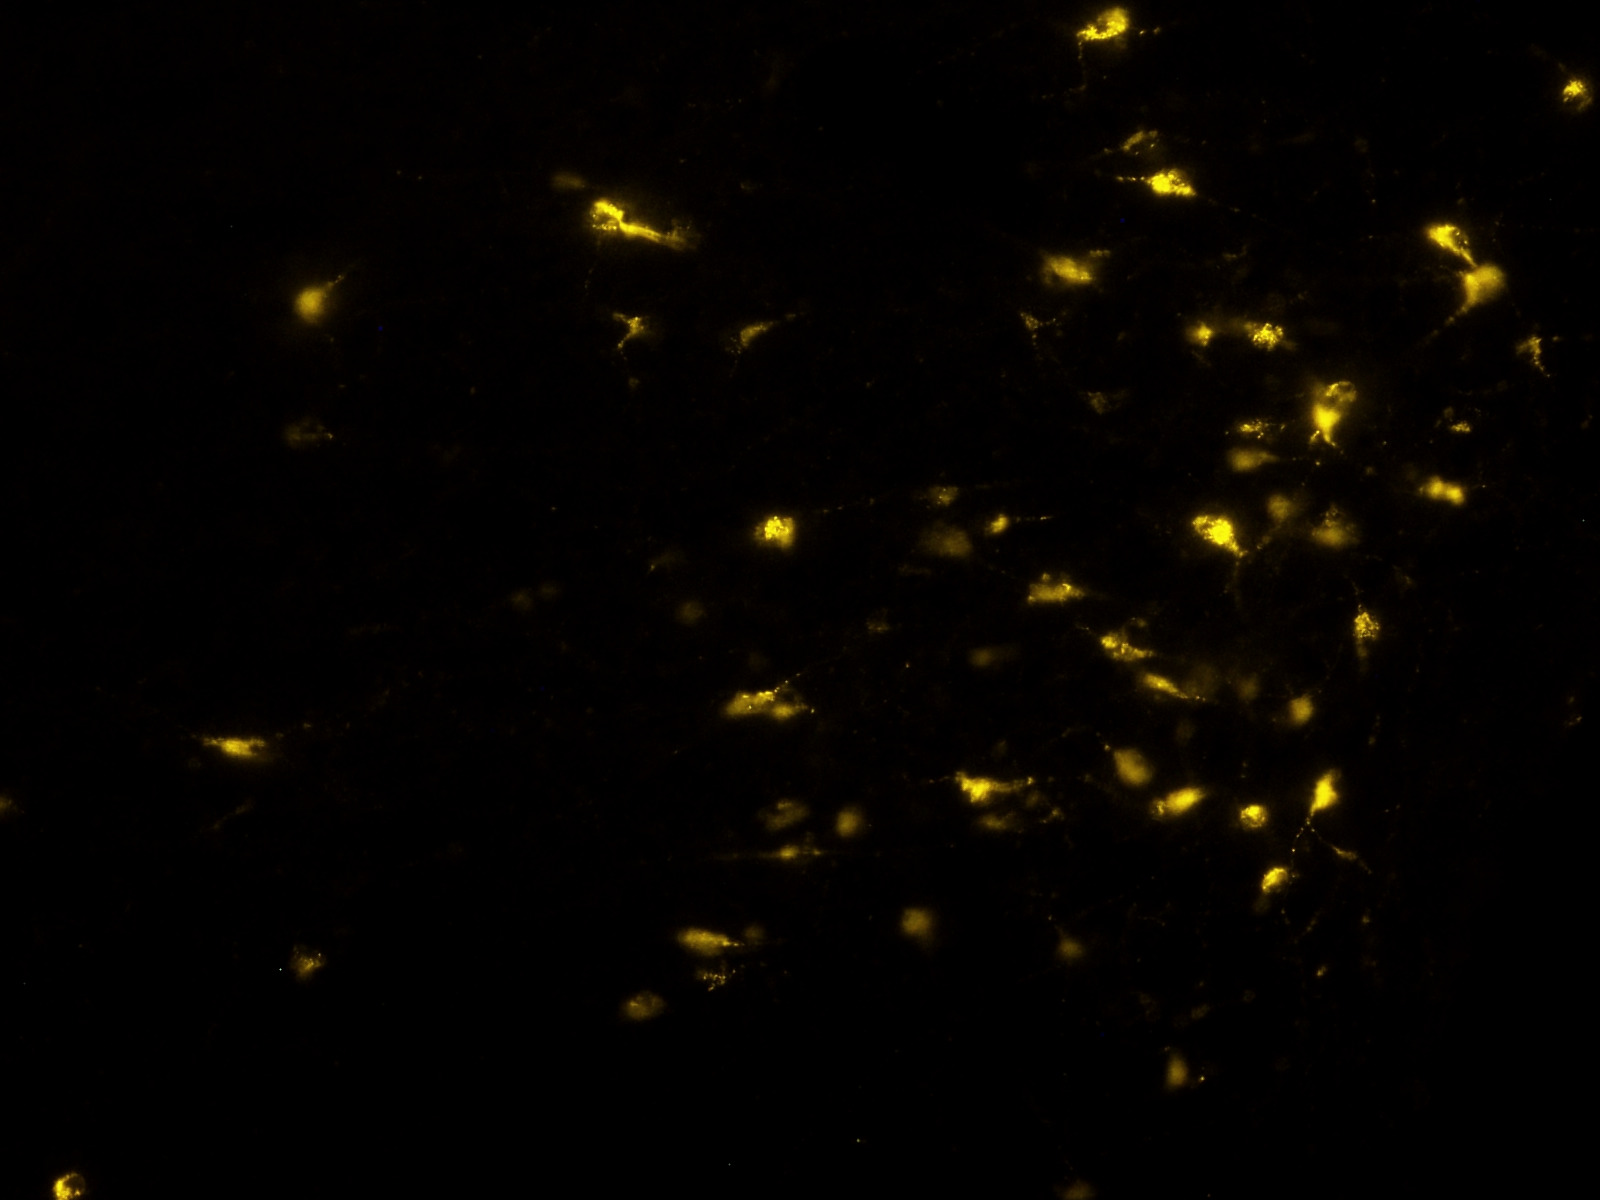
\includegraphics[width=\linewidth]{figures/120_dataset/i_168.jpeg}
\subcaption{dark}\label{fig:dataset:dark}
\end{subfigure}
\begin{subfigure}{0.5\textwidth}
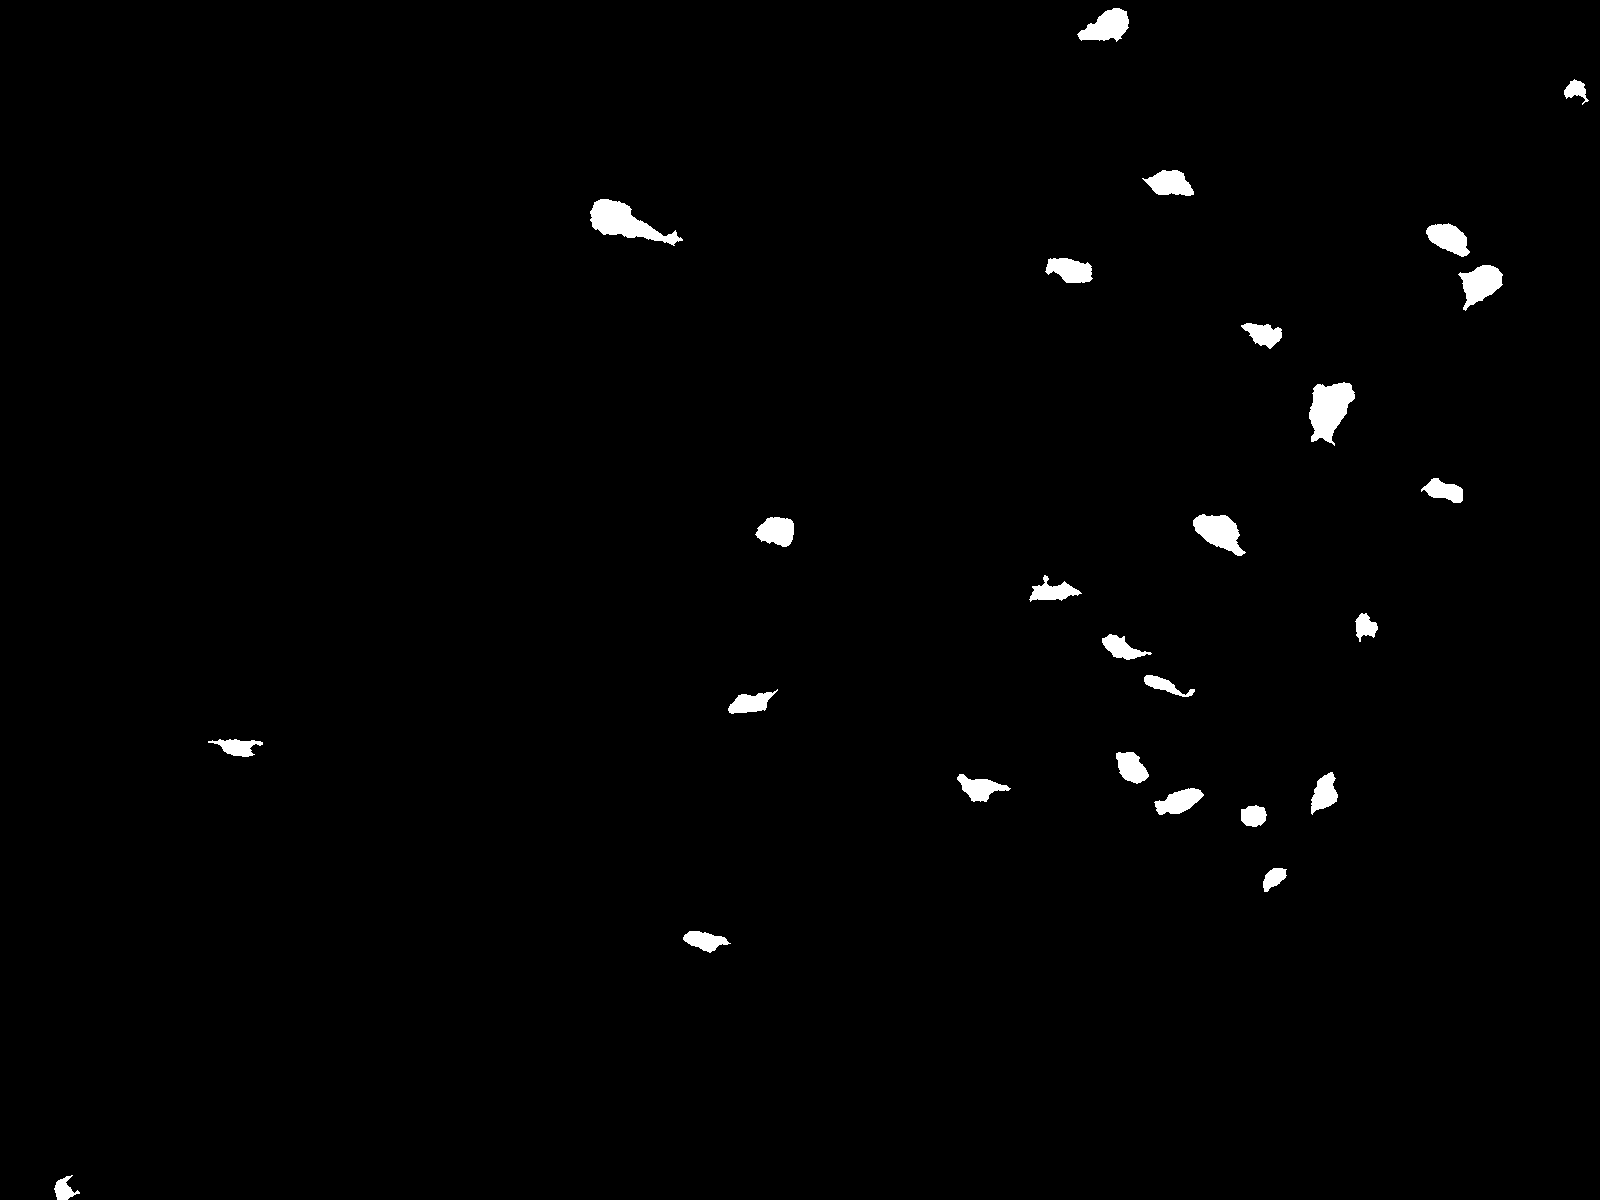
\includegraphics[width=\linewidth]{figures/120_dataset/m_168.png}
\subcaption{mask}\label{fig:dataset:dark_mask}
% \label{fig:dataset:dark}
\end{subfigure}

\begin{subfigure}{0.5\textwidth}
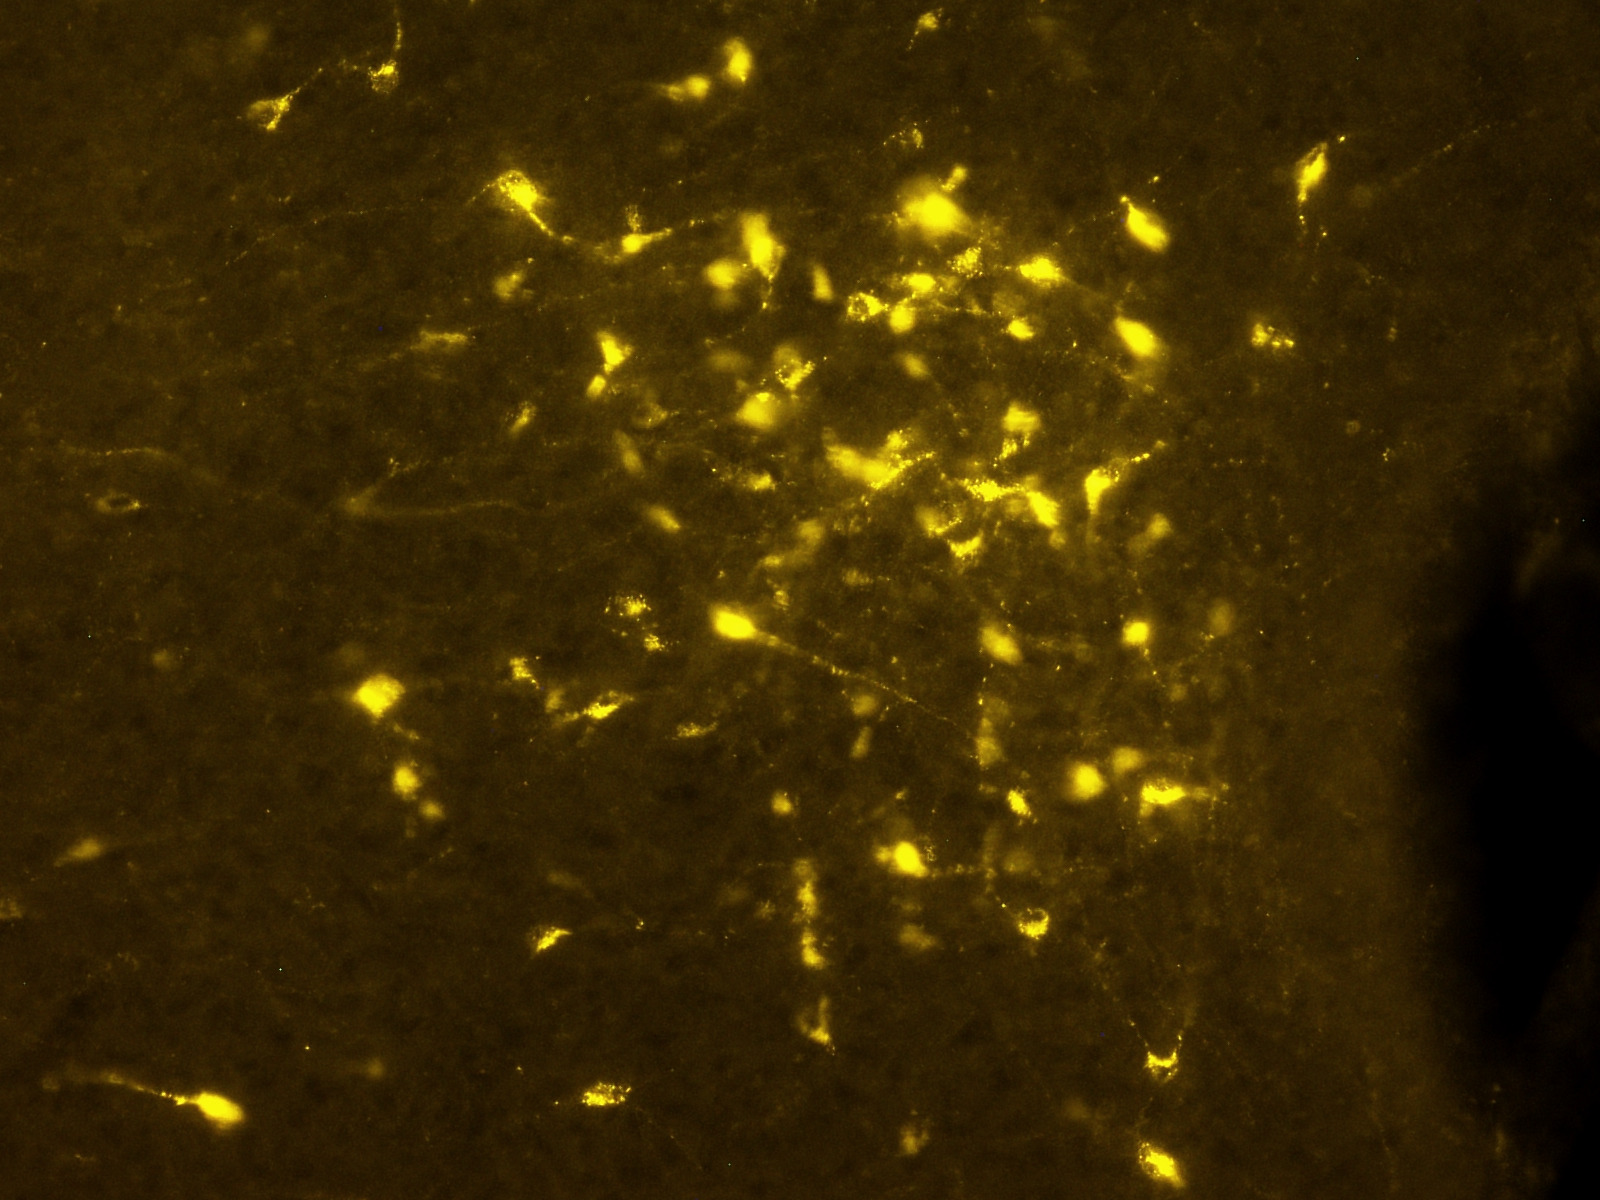
\includegraphics[width=\linewidth]{figures/120_dataset/i_257.jpeg}
\subcaption{bright}\label{fig:dataset:bright}
\end{subfigure}
\begin{subfigure}{0.5\textwidth}
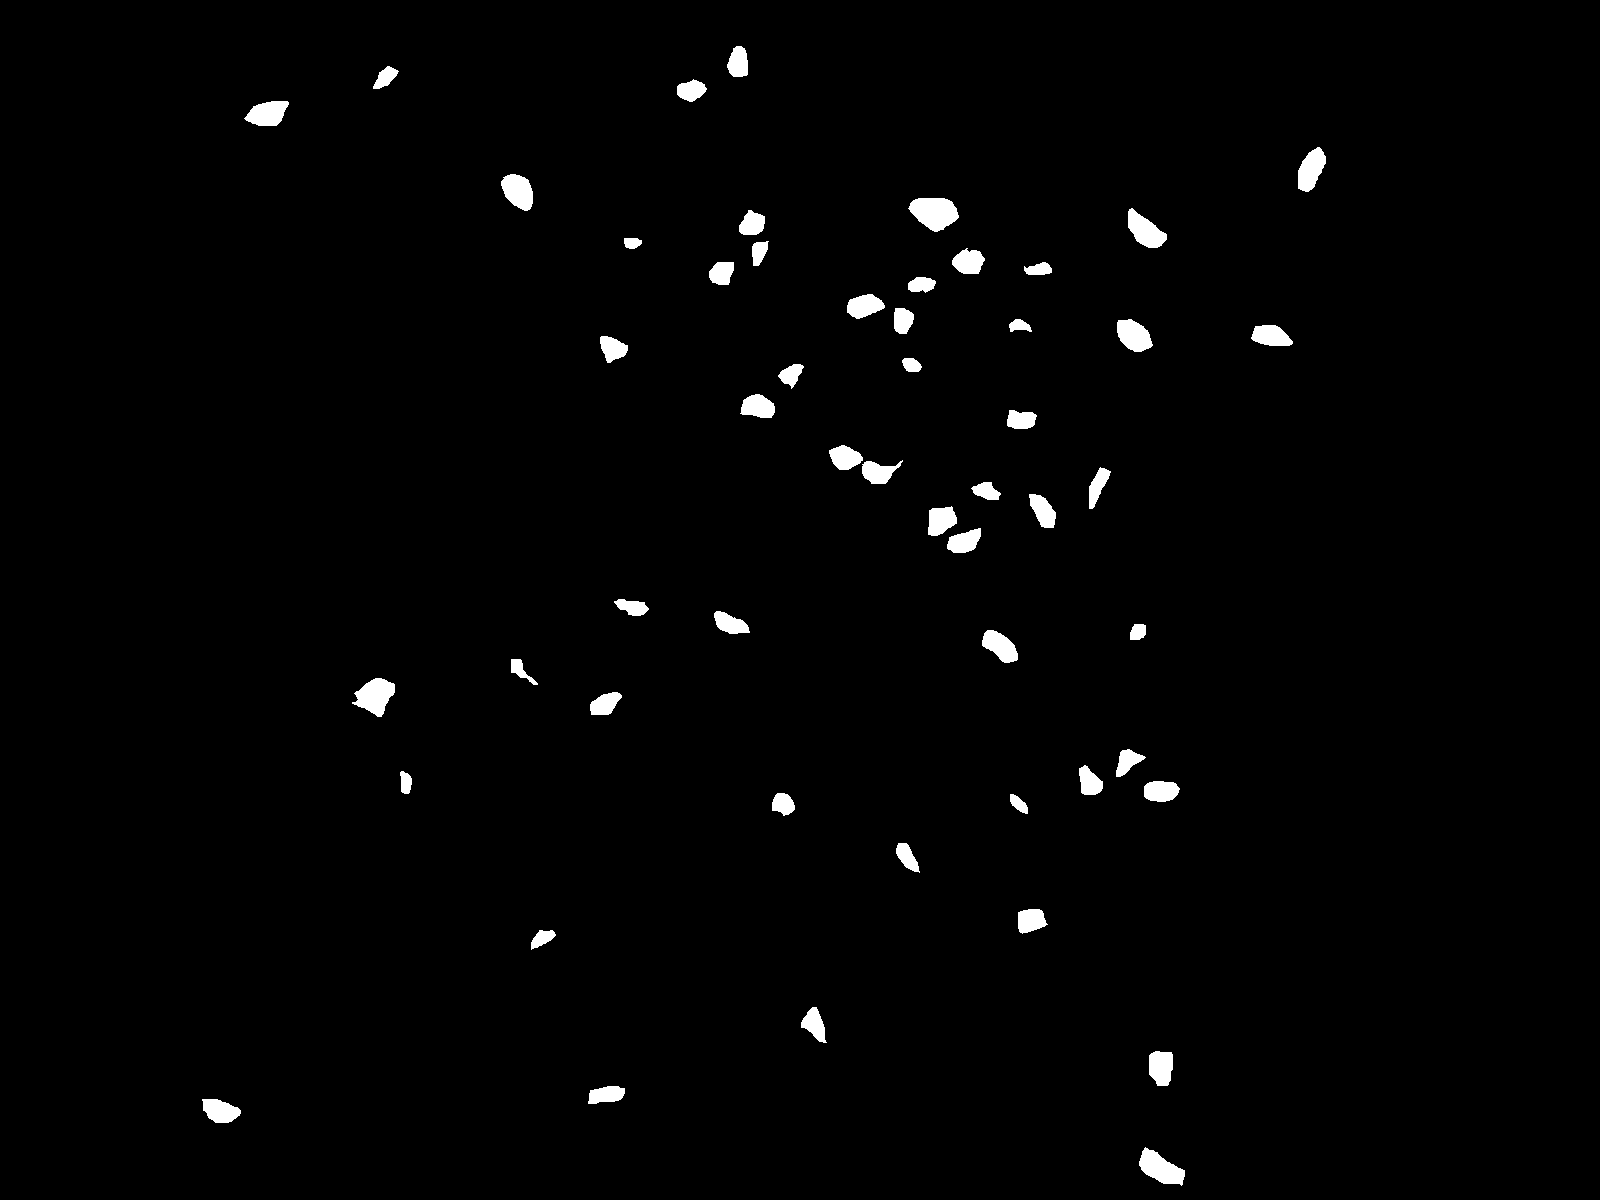
\includegraphics[width=\linewidth]{figures/120_dataset/m_257.png}
\subcaption{mask}\label{fig:dataset:bright_mask}
% \label{fig:dataset:bright}
\end{subfigure}
% \vspace{-0.2cm}
\caption{
\textbf{Sample data}. 
Raw images and corresponding ground-truth masks.
% The original images (left) present neuronal cells of different shape, size and saturation over a background of variable brightness and color.
% The corresponding ground-truth masks used for training (right) depicts cells as white pixels over a black background.
} \label{fig:dataset}
\end{figure}%
% \begin{figure}%[ht]\ContinuedFloat
% \centering
% \begin{subfigure}{0.5\textwidth}
% 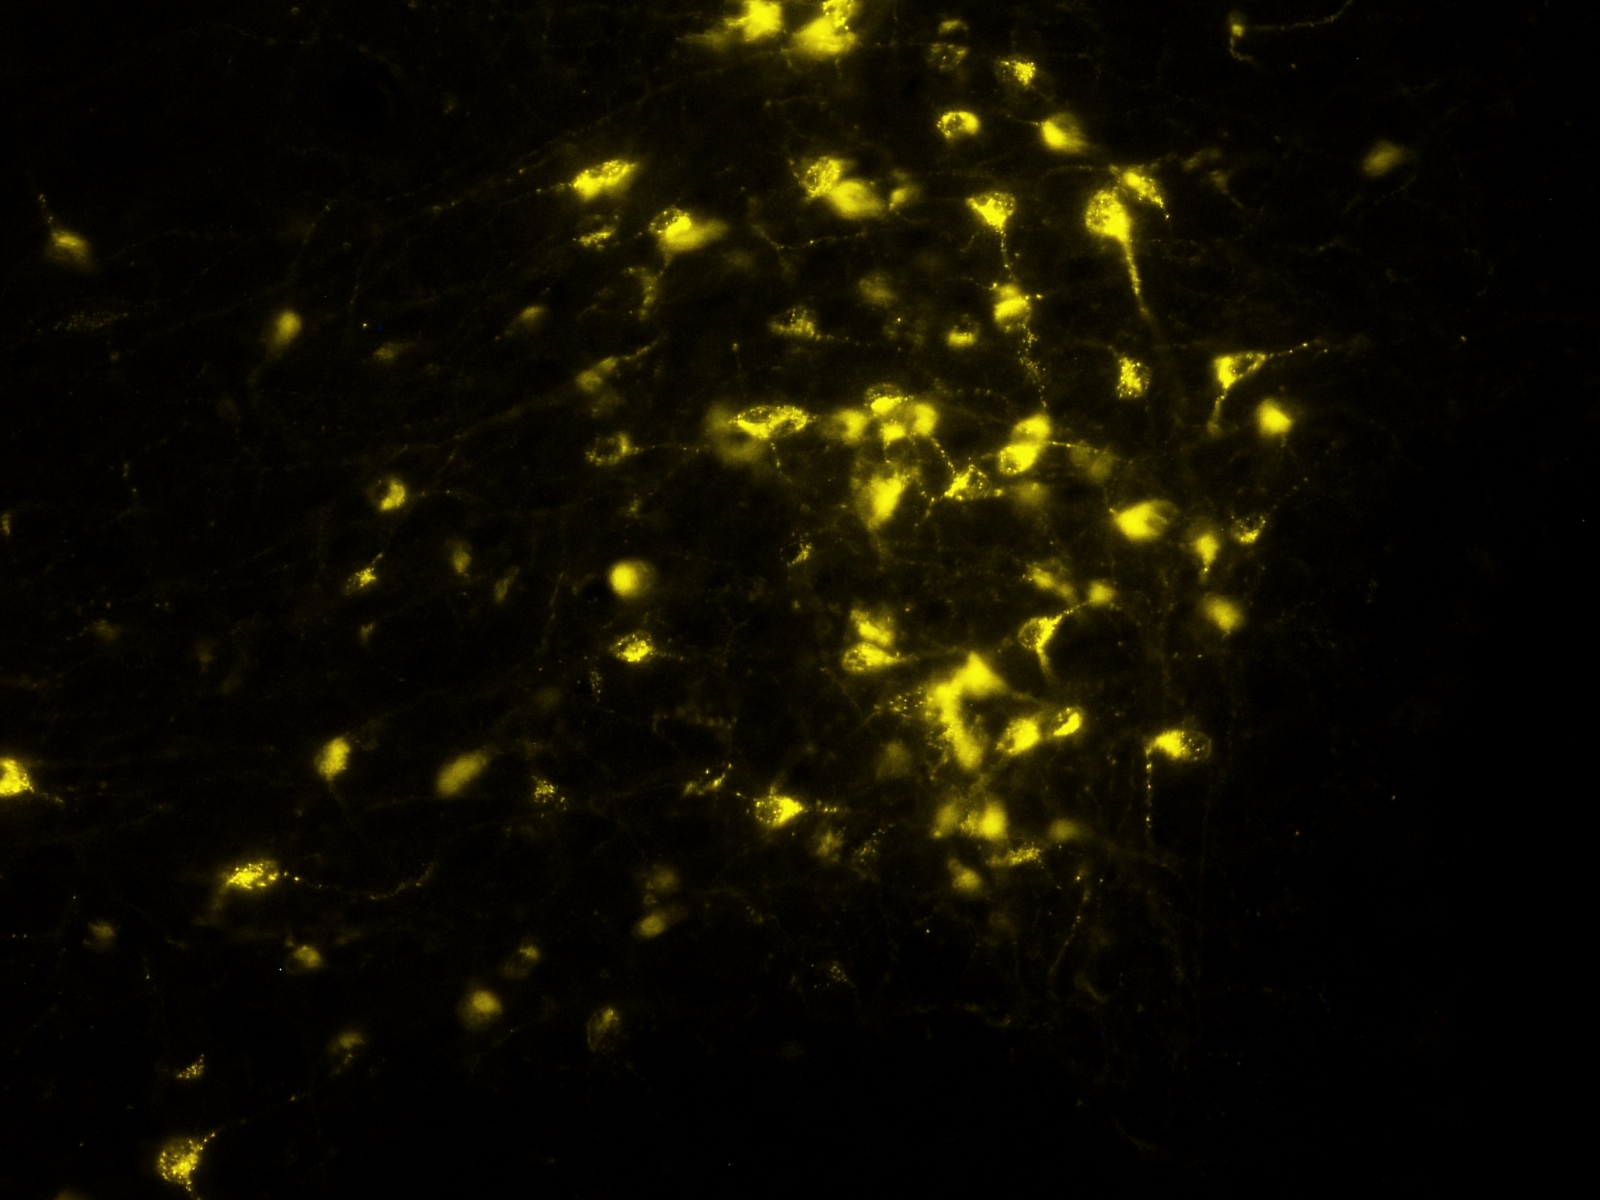
\includegraphics[width=\linewidth]{figures/120_dataset/i_clumping_yellow.png}
% \subcaption{}
% \end{subfigure}%
% \begin{subfigure}{0.5\textwidth}
% 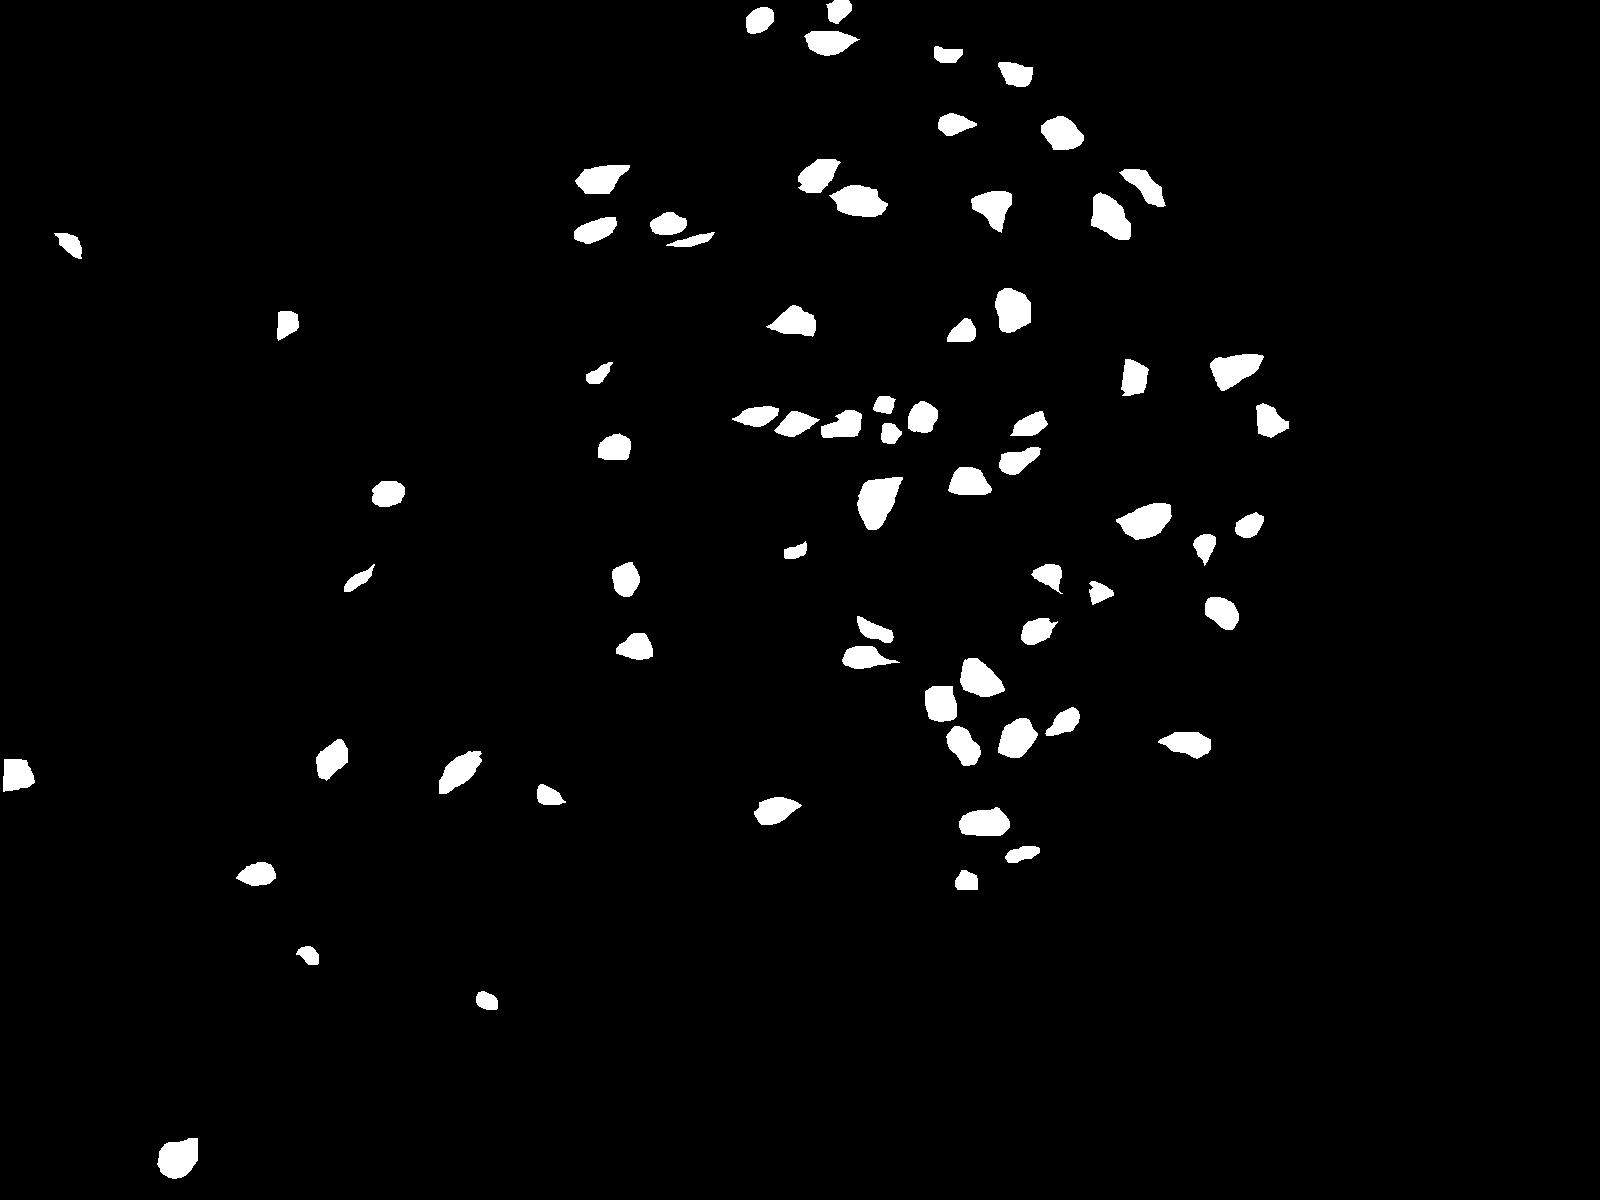
\includegraphics[width=\linewidth]{figures/120_dataset/m_clumping_yellow.png}
% \subcaption{}
% \label{fig:artifacts:clumping}
% \end{subfigure}

% \begin{subfigure}{0.5\textwidth}
% 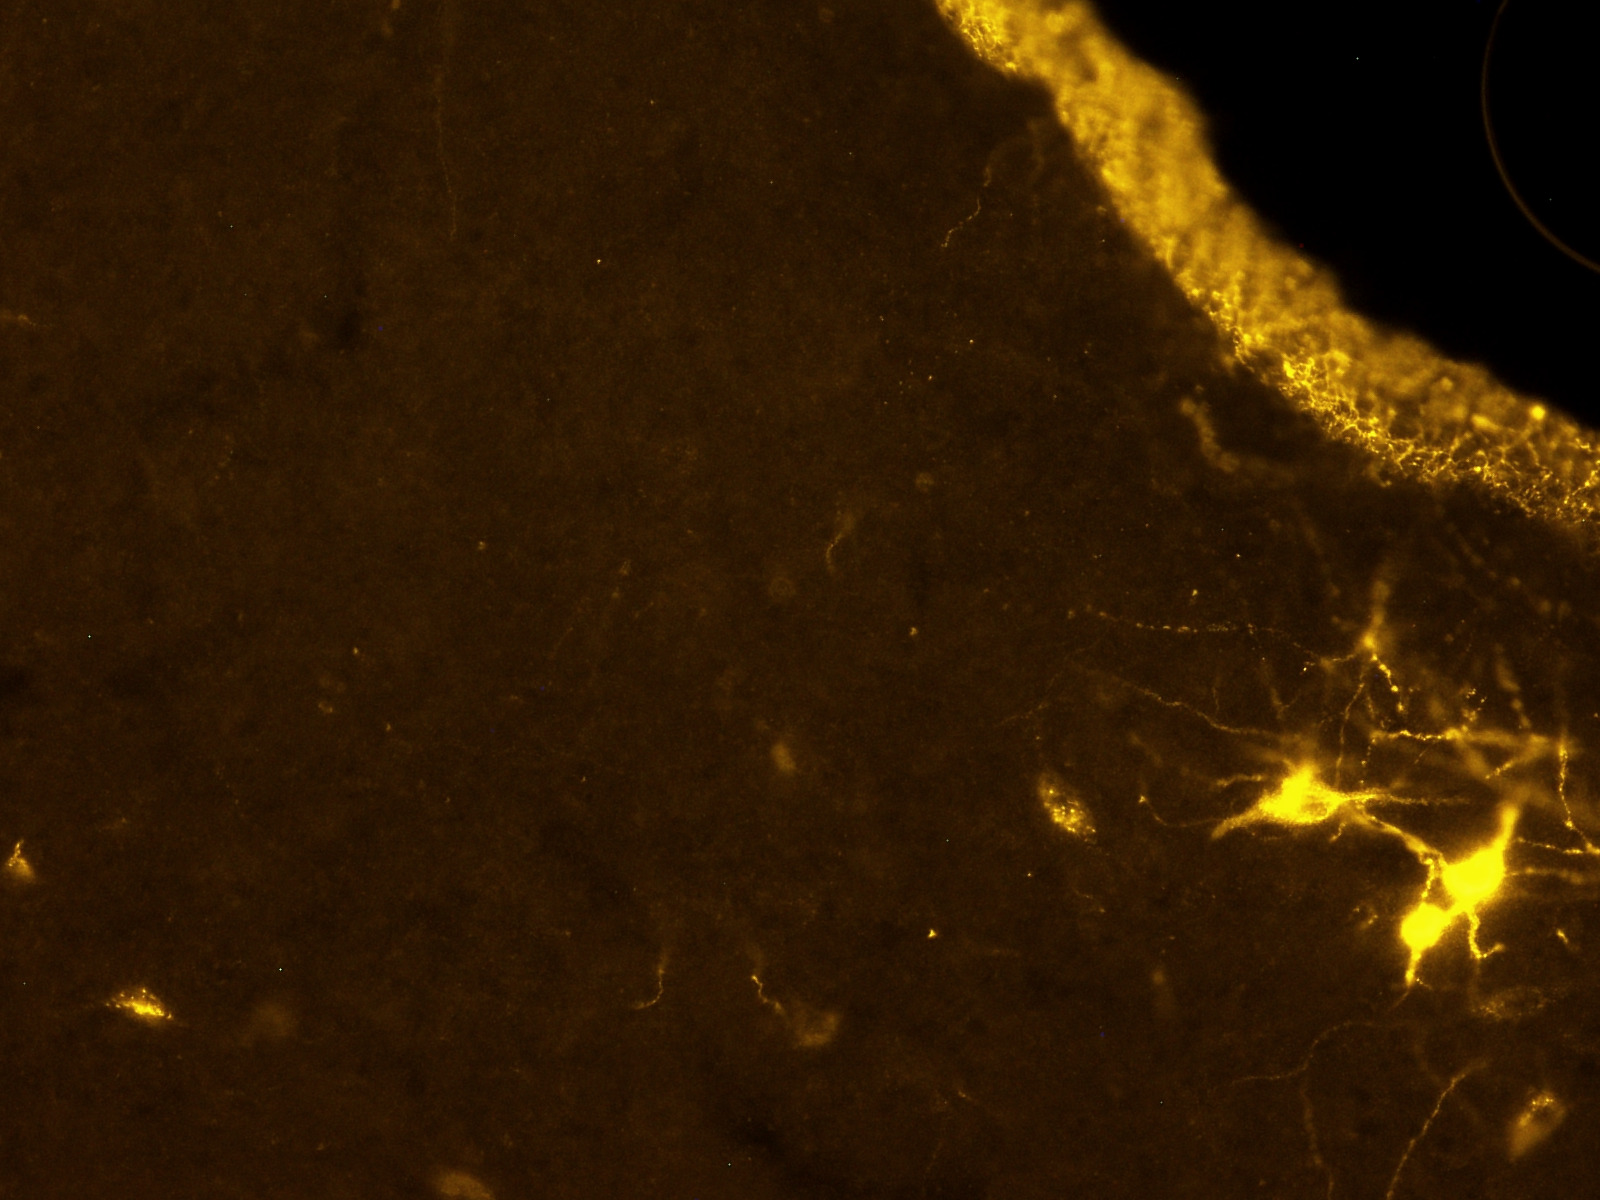
\includegraphics[width=\linewidth]{figures/120_dataset/i_252.jpeg}
% \subcaption{}
% \end{subfigure}%
% \begin{subfigure}{0.5\textwidth}
% 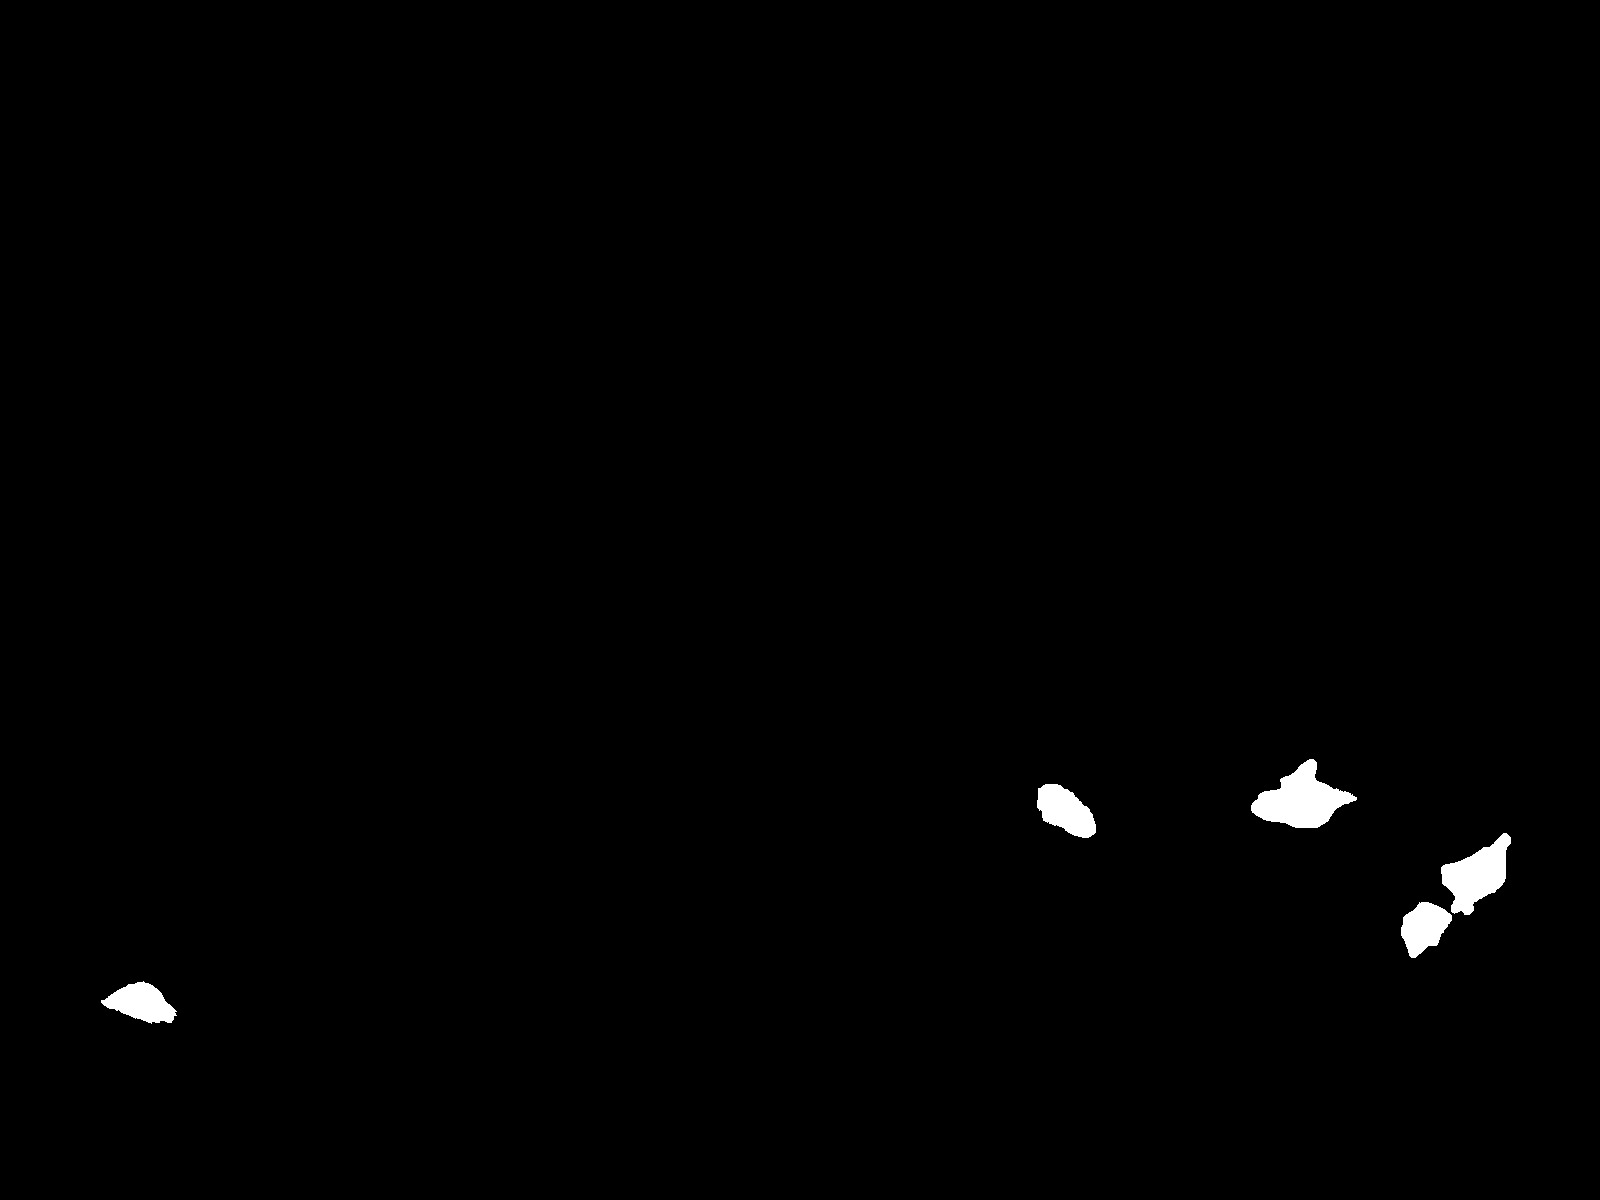
\includegraphics[width=\linewidth]{figures/120_dataset/m_252.jpeg}
% \subcaption{}
% \label{fig:artifacts:stripe}
% \end{subfigure}%

% \begin{subfigure}{0.5\textwidth}
% 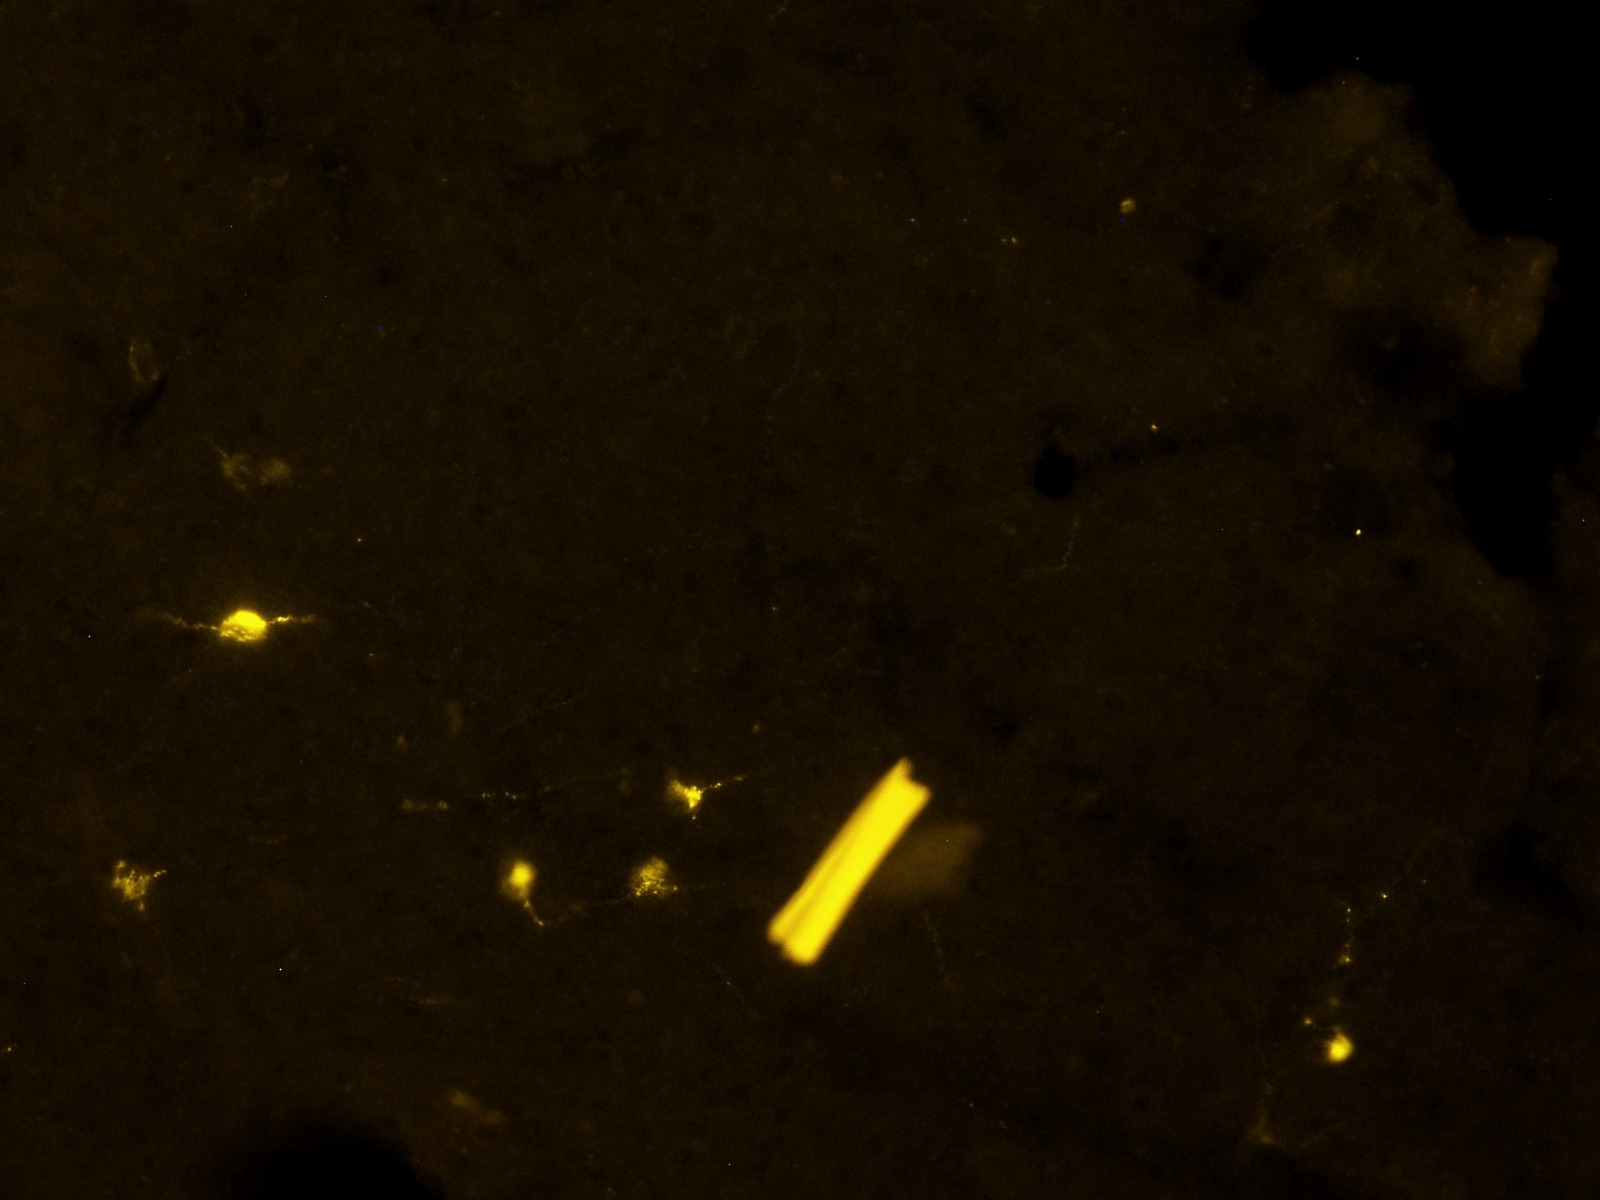
\includegraphics[width=\linewidth]{figures/120_dataset/i_maccherone.jpeg}
% \subcaption{}
% \end{subfigure}%
% \begin{subfigure}{0.5\textwidth}
% 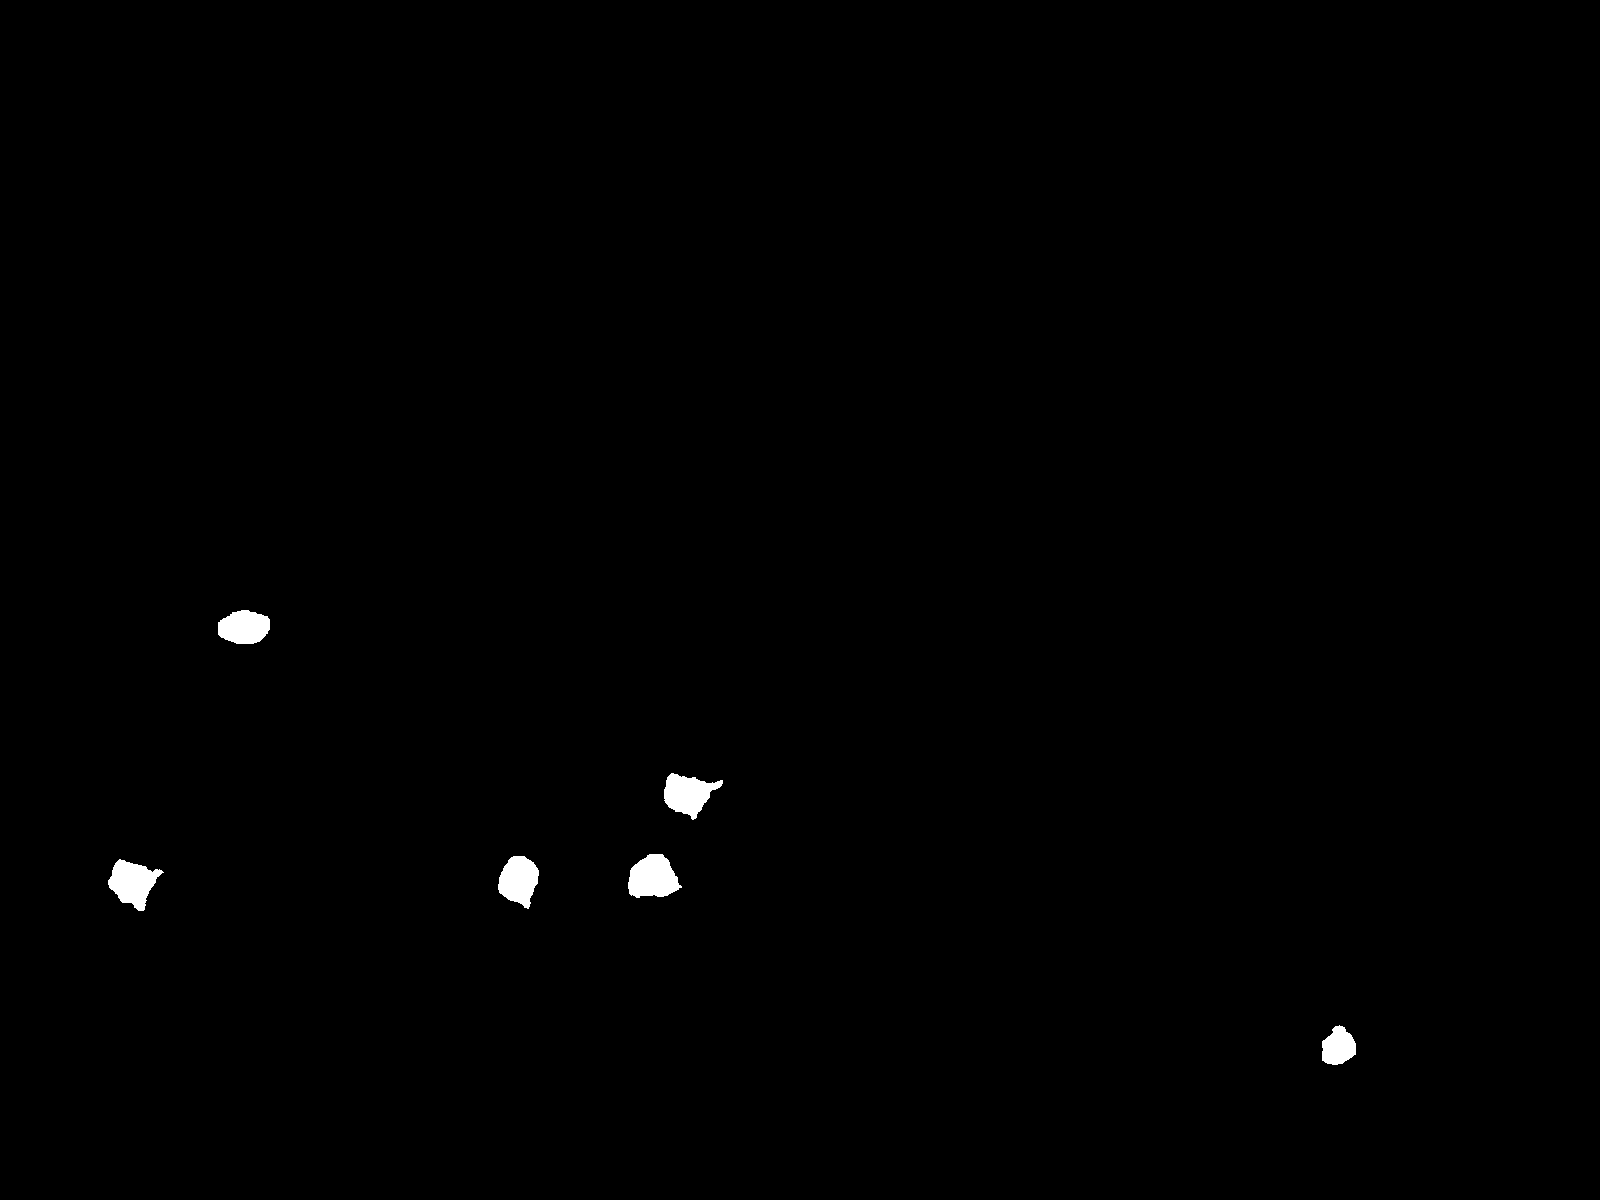
\includegraphics[width=\linewidth]{figures/120_dataset/m_maccherone.png}
% \subcaption{}
% \label{fig:artifacts:macaroon}
% \end{subfigure}
% \vspace{-0.2cm}
% \caption{
% \textbf{Artifacts and challenges}. Neuronal cells appear of different shape, size and saturation over a background of variable brightness and color.
% %%rephrase
% % \textbf{Sample data}. In the original images (left), the neuronal cells of interest appear as yellow spots over a background of variable brightness and color. They exhibit a large variability in terms of shape, size and saturation, which makes them hard to distinguish from artifacts and similar biological structures that are not of interest.
% % The corresponding ground-truth masks used for training (right) depicts cells as white pixels over a black background.
% } 
% \label{fig:artifacts}
% \end{figure}
% \clearpage
% \restoregeometry

% \savegeometry{origigeom}
% \clearpage
% \newgeometry{lmargin=0.5cm}
% \begin{figure}%[ht]\ContinuedFloat
% \centering
% \begin{subfigure}{0.55\textwidth}
% % \subfloat[]{
% 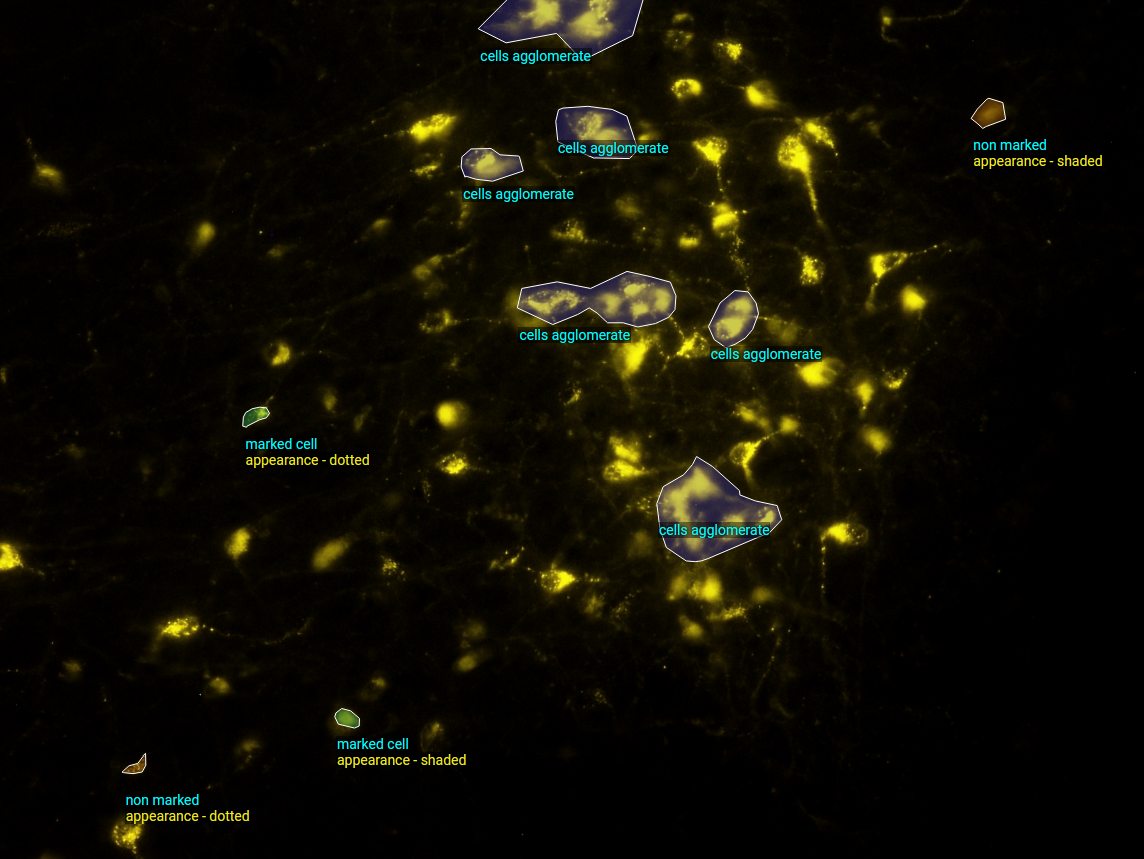
\includegraphics[width=\linewidth]{figures/120_dataset/annotated_i_clumping.png}
% \label{fig:artifacts:clumping}
% % }
% \subcaption{}
% \end{subfigure}%
% \begin{subfigure}{0.55\textwidth}
% % \subfloat[]{
% 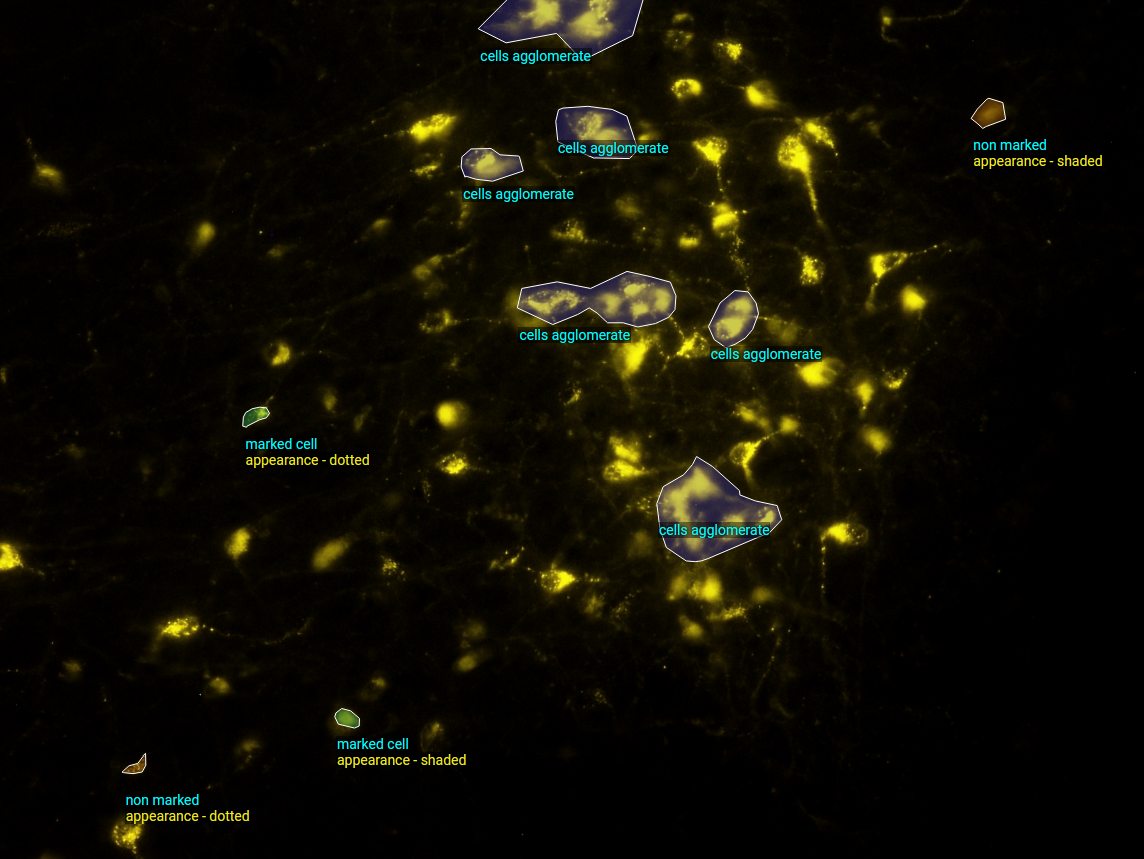
\includegraphics[width=\linewidth]{figures/120_dataset/annotated_i_clumping.png}
% \label{fig:artifacts:clumping}
% % }
% \subcaption{}
% \end{subfigure}
% \centering
% \begin{subfigure}{0.55\textwidth}
% % \subfloat[]{
% 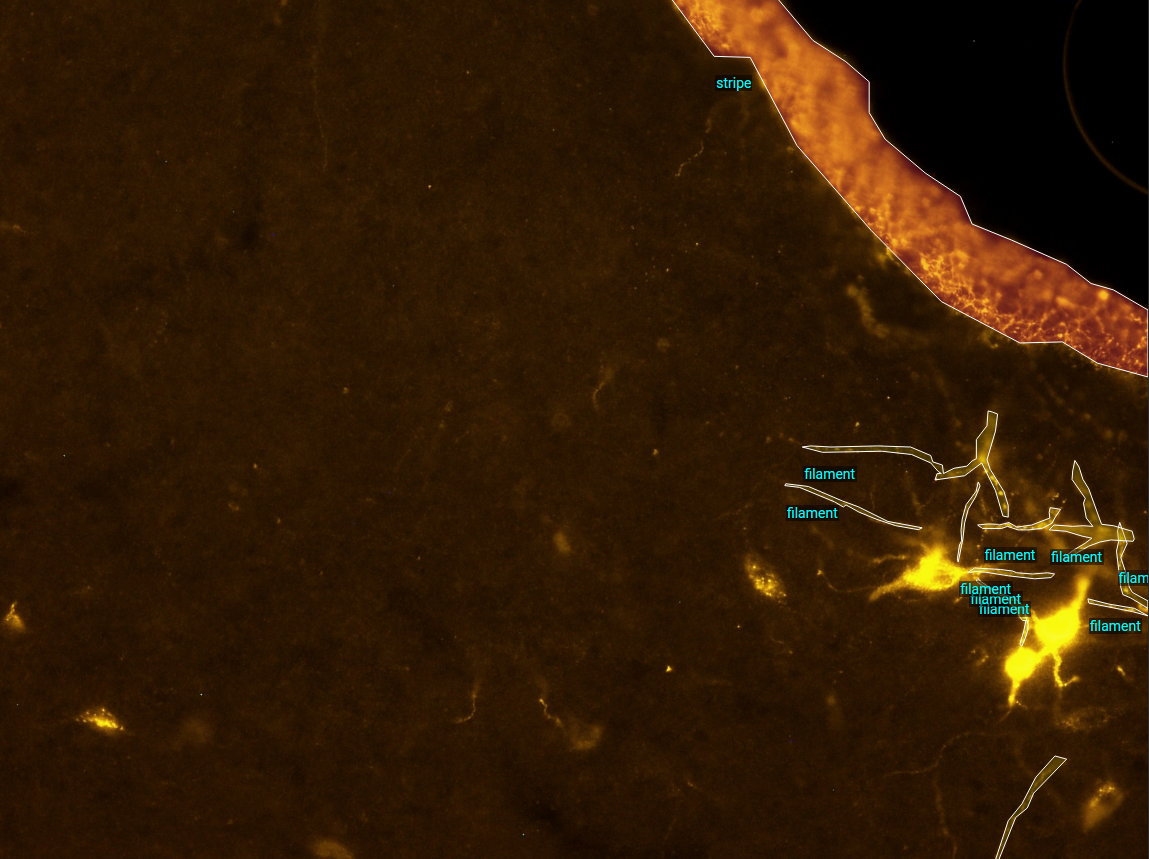
\includegraphics[width=\linewidth]{figures/120_dataset/annotated_i_stripe.png}
% \label{fig:artifacts:stripe}
% % }
% \subcaption{}
% \end{subfigure}%
% \begin{subfigure}{0.55\textwidth}
% % \subfloat[]{
% 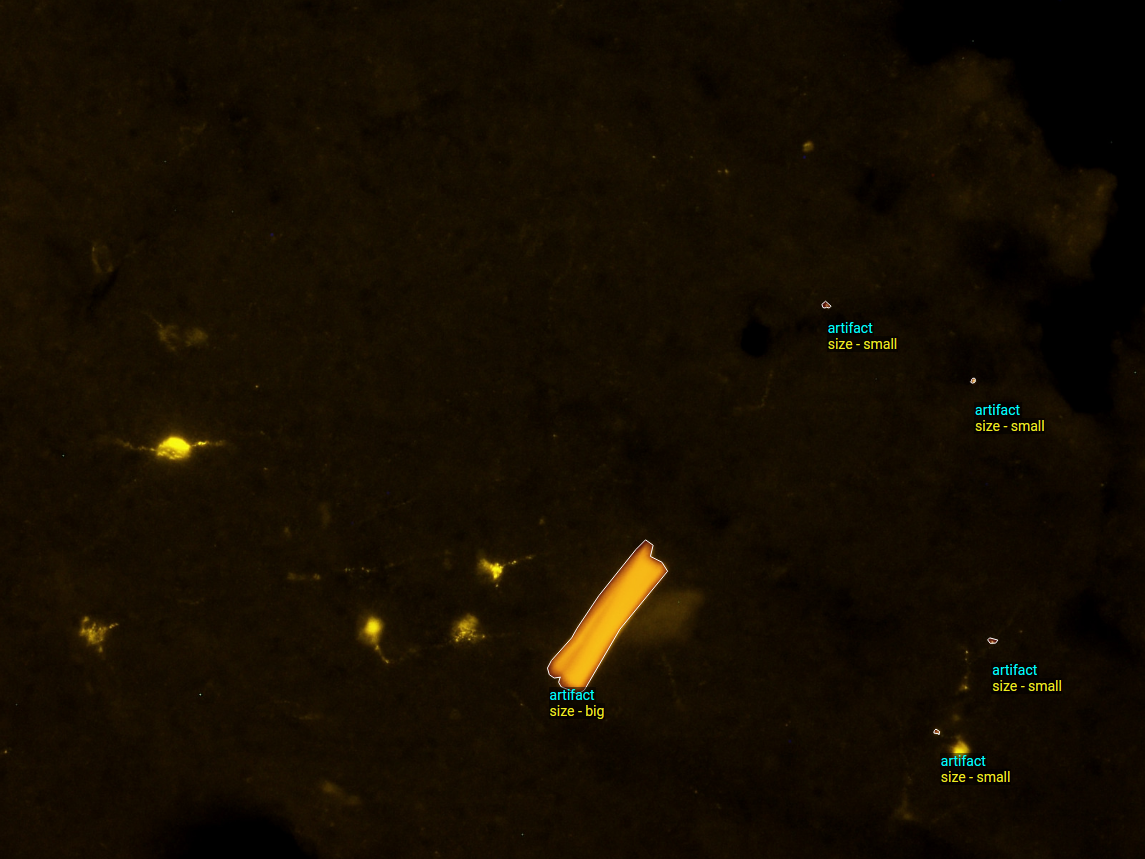
\includegraphics[width=\linewidth]{figures/120_dataset/annotated_i_macaroon.png}
% \label{fig:artifacts:macaroon}
% % }
% \subcaption{}
% \end{subfigure}

% \vspace{-0.2cm}
% \caption{
% \textbf{Artifacts and challenges}. Neuronal cells appear of different shape, size and saturation over a background of variable brightness and color.
% %%rephrase
% % \textbf{Sample data}. In the original images (left), the neuronal cells of interest appear as yellow spots over a background of variable brightness and color. They exhibit a large variability in terms of shape, size and saturation, which makes them hard to distinguish from artifacts and similar biological structures that are not of interest.
% % The corresponding ground-truth masks used for training (right) depicts cells as white pixels over a black background.
% } 
% \label{fig:artifacts2}
% \end{figure}
% \clearpage
% \restoregeometry

The \textbf{Fluorescent Neuronal Cells} dataset \cite{clissa2021fluocells} consists of 283 
% high-resolution 
pictures 
% (1600$\times$1200 pixels) 
of mice brain slices and the corresponding ground-truth labels.
In order to acquire these images, the mice were subjected to controlled experimental conditions, and a monosynaptic retrograde tracer (b-subunit of Cholera Toxin, CTb) was surgically injected into brain tissues to highlight the neurons connected to the injection site
%projecting to the injection site
\cite{hitrec2019neural}.
Specimens of brain slices were then observed through  
a fluorescence microscope configured to select the narrow wavelength of light emitted by a fluorophore (of a yellow/orange color) associated with the tracer.
Hence, the resultant images depict neurons of interest as
% objects of different size and shape appearing as 
yellow-ish spots
% of variable brightness and saturation 
over a composite, generally darker background
% (\cref{fig:dataset,fig:artifacts}).
(\cref{fig:dataset:empty,fig:dataset:dark,fig:dataset:bright}).

% Although many efforts were made to stabilize the acquisition procedure, the images present several relevant challenges for the detection task. 
% For example, the variability in brightness and contrast causes some fickleness in the pictures overall appearance (cf. \cref{fig:dataset:dark,fig:dataset:bright}).  
% Also, the cells themselves exhibit varying saturation levels due to the natural fluctuation of the fluorescent emission properties (cf. \cref{fig:dataset:dark,fig:artifacts:clumping}).
% Moreover, the substructures of interest have a fluid nature. This implies that the size and shape of the stained cells may change significantly (see \cref{fig:artifacts:clumping}, right), making it even harder to discriminate between them and the background. 
% Combined to that, artifacts (\cref{fig:artifacts:stripe,fig:artifacts:macaroon}), bright biological structures -- like neurons' filaments -- (\cref{fig:artifacts:stripe}) and non-marked cells similar to the stained ones handicap the recognition task. 
% Last but not least, another source of complexity is the broad shift in the number of target cells from image to image.
% Indeed, the total counts range from no stained cells (\cref{fig:dataset:empty}) to several dozens clumping together (\cref{fig:artifacts:clumping}). 
% As a consequence, this requires a model with both high precision -- to prevent false positives in the former case -- and high recall -- since considering two or more touching neurons only once produces false negatives.
% % In the former case, the model needs high precision in order to prevent false positives. The latter, instead,
% % requires high recall since considering two or more touching neurons only once produces false negatives. 

% By and large, all of these factors make the recognition and counting tasks more problematic and complicate the model training.
% Likewise, these challenges hinder model evaluation as the interpretation of such borderline cases becomes subjective.
